\section{Results and Discussion}
\label{Chap:Al/Vac:section:RD}
\subsection{Cluster Searching Algorithm}

In order to better analyzing our results, we have to use a visualization method to characterize clusters. A cluster is a set of connected atoms, each of which is within the range of one or more other atoms from the same cluster. Thus, any two atoms from the same cluster are connected by a continuous path consisting of steps fulfilling the selected neighboring criterion. Adversely, two atoms are not considered in the same cluster if there is no continuous path on the neighbor network leading from one particle to the other. We choose between the distance-based neighbor criterion, in which case two atoms are considered neighbors if they are within the neighbor list of each other. However, in our case, all the atoms are on lattice, so the method described above does not work. It will simply find one huge cluster containing all the atoms. Therefore, we use the method described in Algorithm. \ref{algo:cluster}. We show one typical results in Fig. \ref{Chap:Al/Vac:fig:illu_cluster}. The only top ten clusters are shown. And as you can see, dark red and orange clusters are almost connected. They share one Al atom in common. In that case we treat them as two clusters. Otherwise, if Al atoms are treated like bridges, then most of the atoms in the supercell will be connected as one huge cluster, which is not desired.


\begin{figure}[!htb]
  \centering
  \begin{minipage}{.75\linewidth}
    \begin{algorithm}[H]
      \caption{Cluster Searching Algorithm}\label{algo:cluster}
      \begin{algorithmic}[1]
        \State remove all the solvent atoms (Al for example).
        \State assign an initial cluster id, ($cid = -1$), to all the atoms.
        \State set $count = 0$.
        \For {i in all the solute atoms}
          \If {$cid_i = -1$}
            \State set $cid_i = count$.
            \State \ac{BFS} in the neighbor list of atom i to find other solute atoms and set their $cid = count$.
            \State add their first nearest neighbor solvent atoms (Al for example) back and set their $cid = count$.
            \State $count += 1$.
          \EndIf
        \EndFor
        \State then clusters can be sorted according to any customized methods, by cluster size, element ratios for examples.
      \end{algorithmic}
    \end{algorithm}
  \end{minipage}
\end{figure}


\begingroup
\begin{figure}[!ht]
  \centering
  \subfigure[]{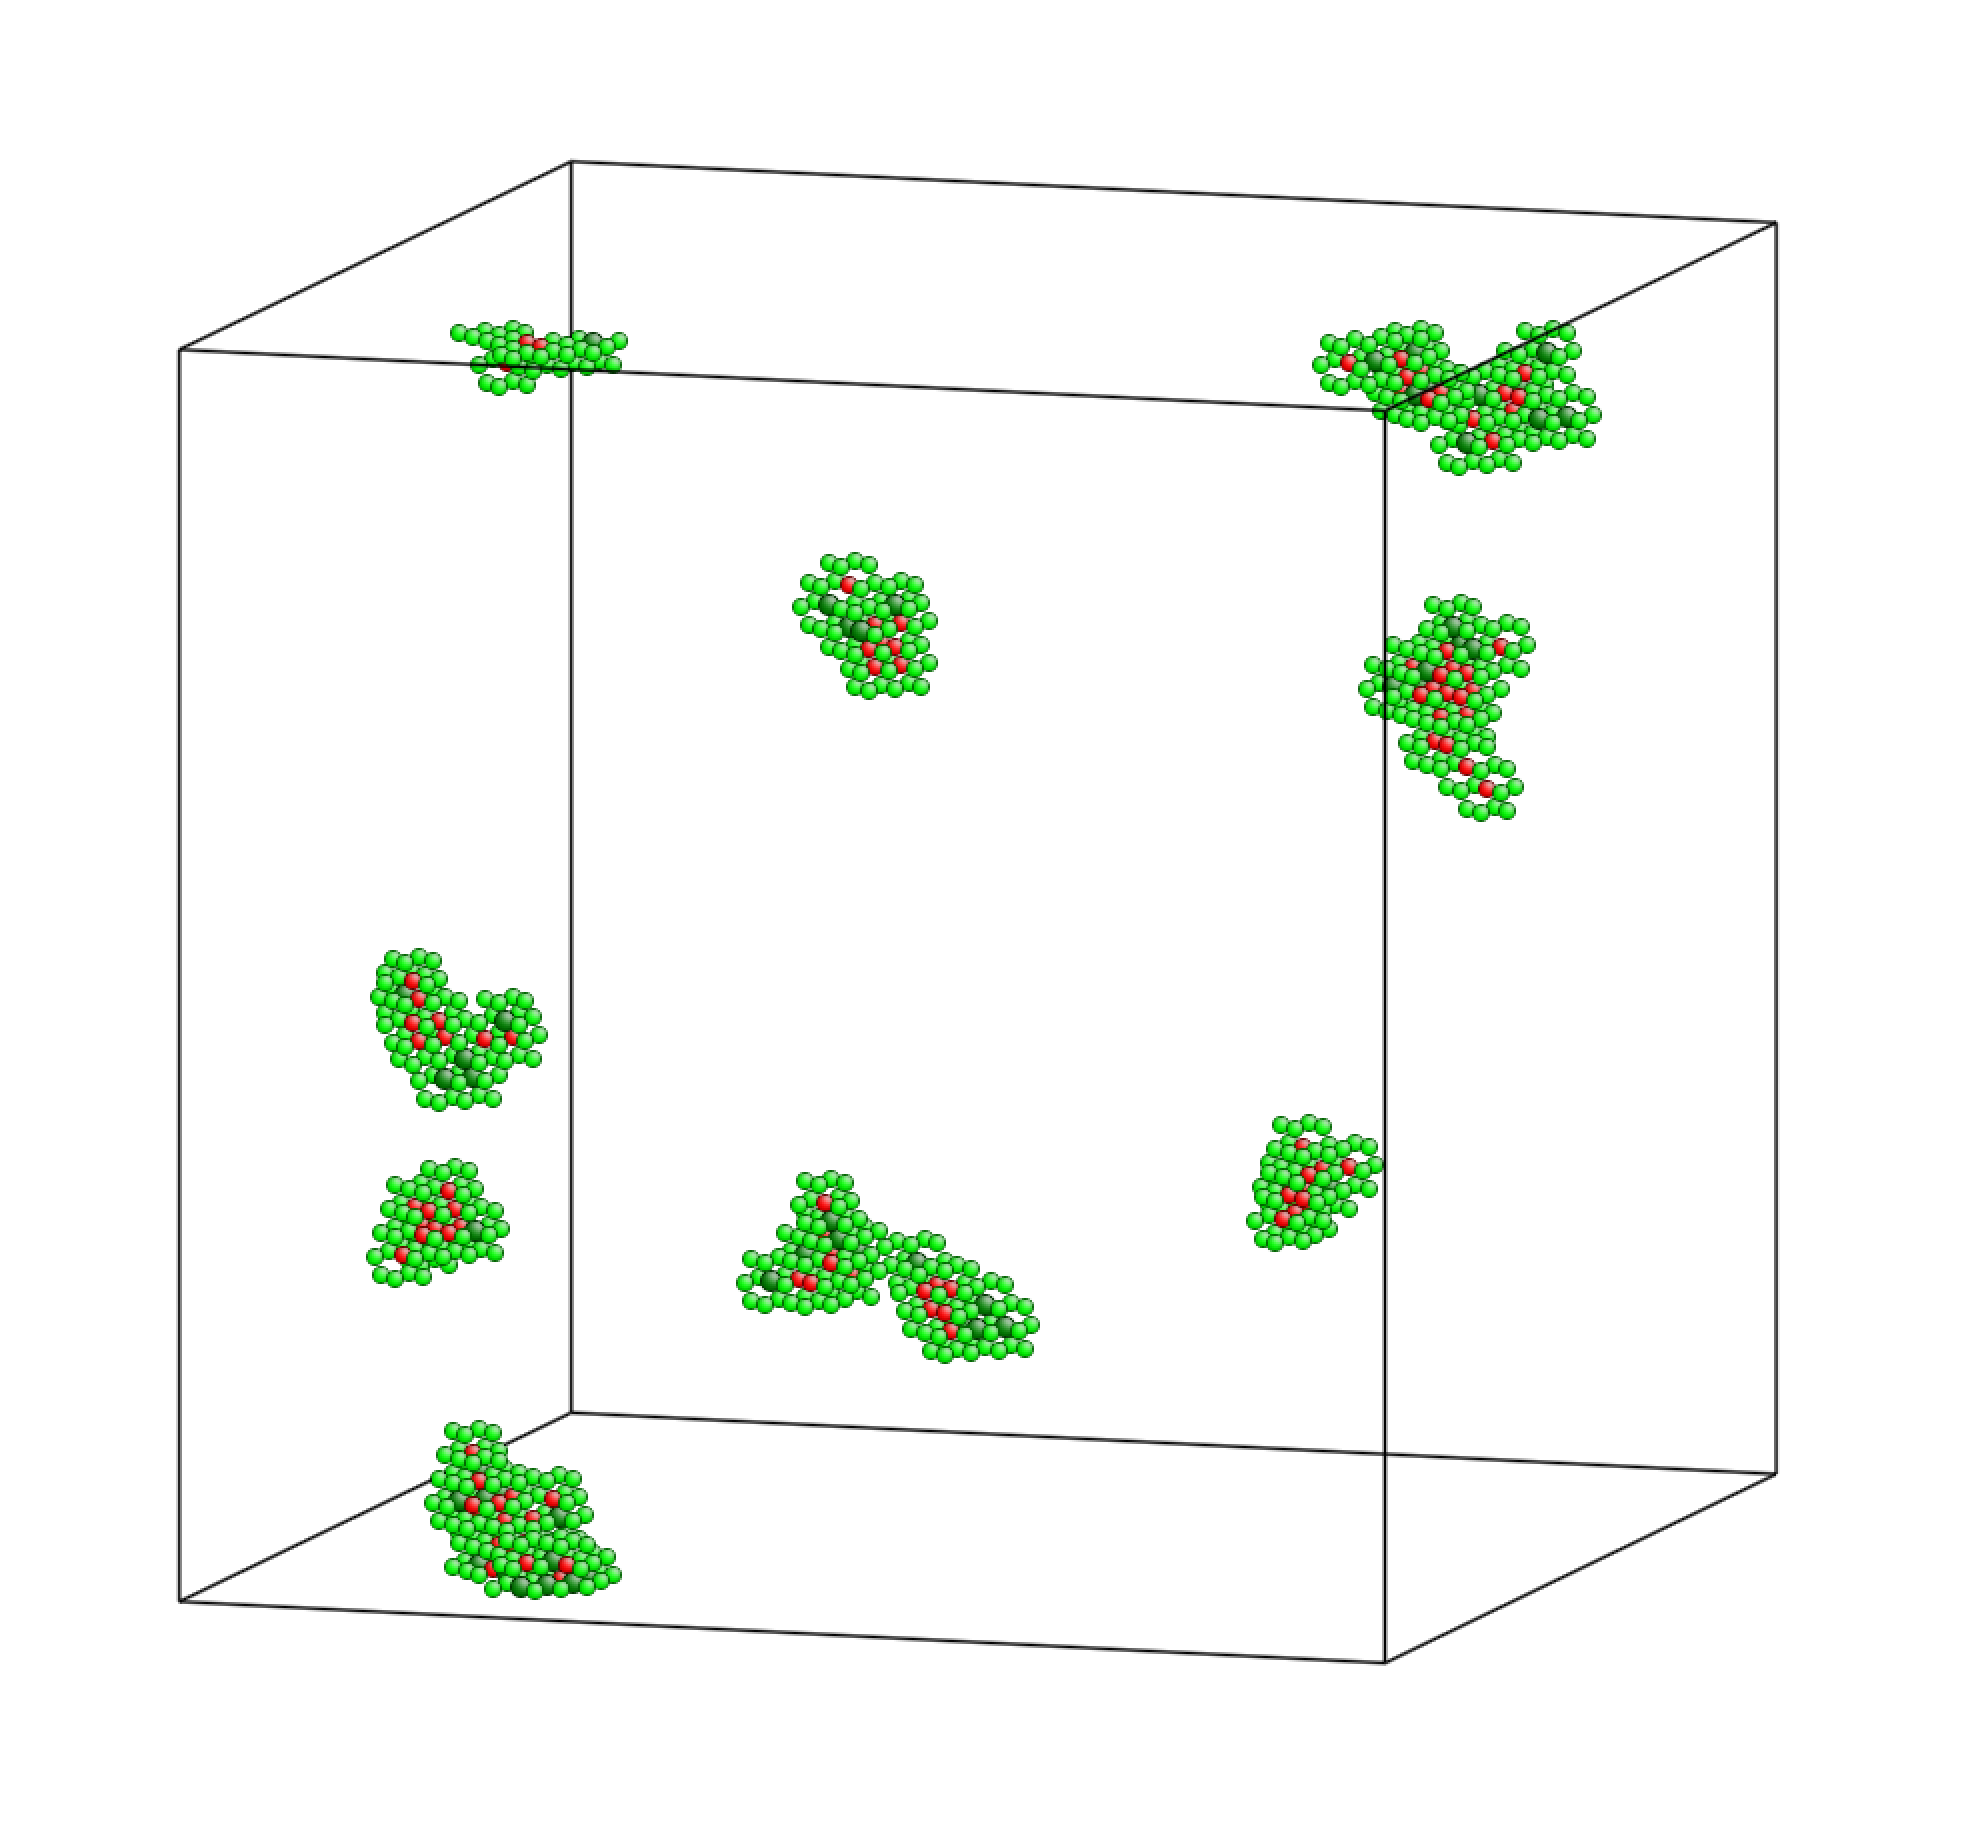
\includegraphics[width=0.49\linewidth]{Chap5/plots/cluster_illu_1.png}}
  \subfigure[]{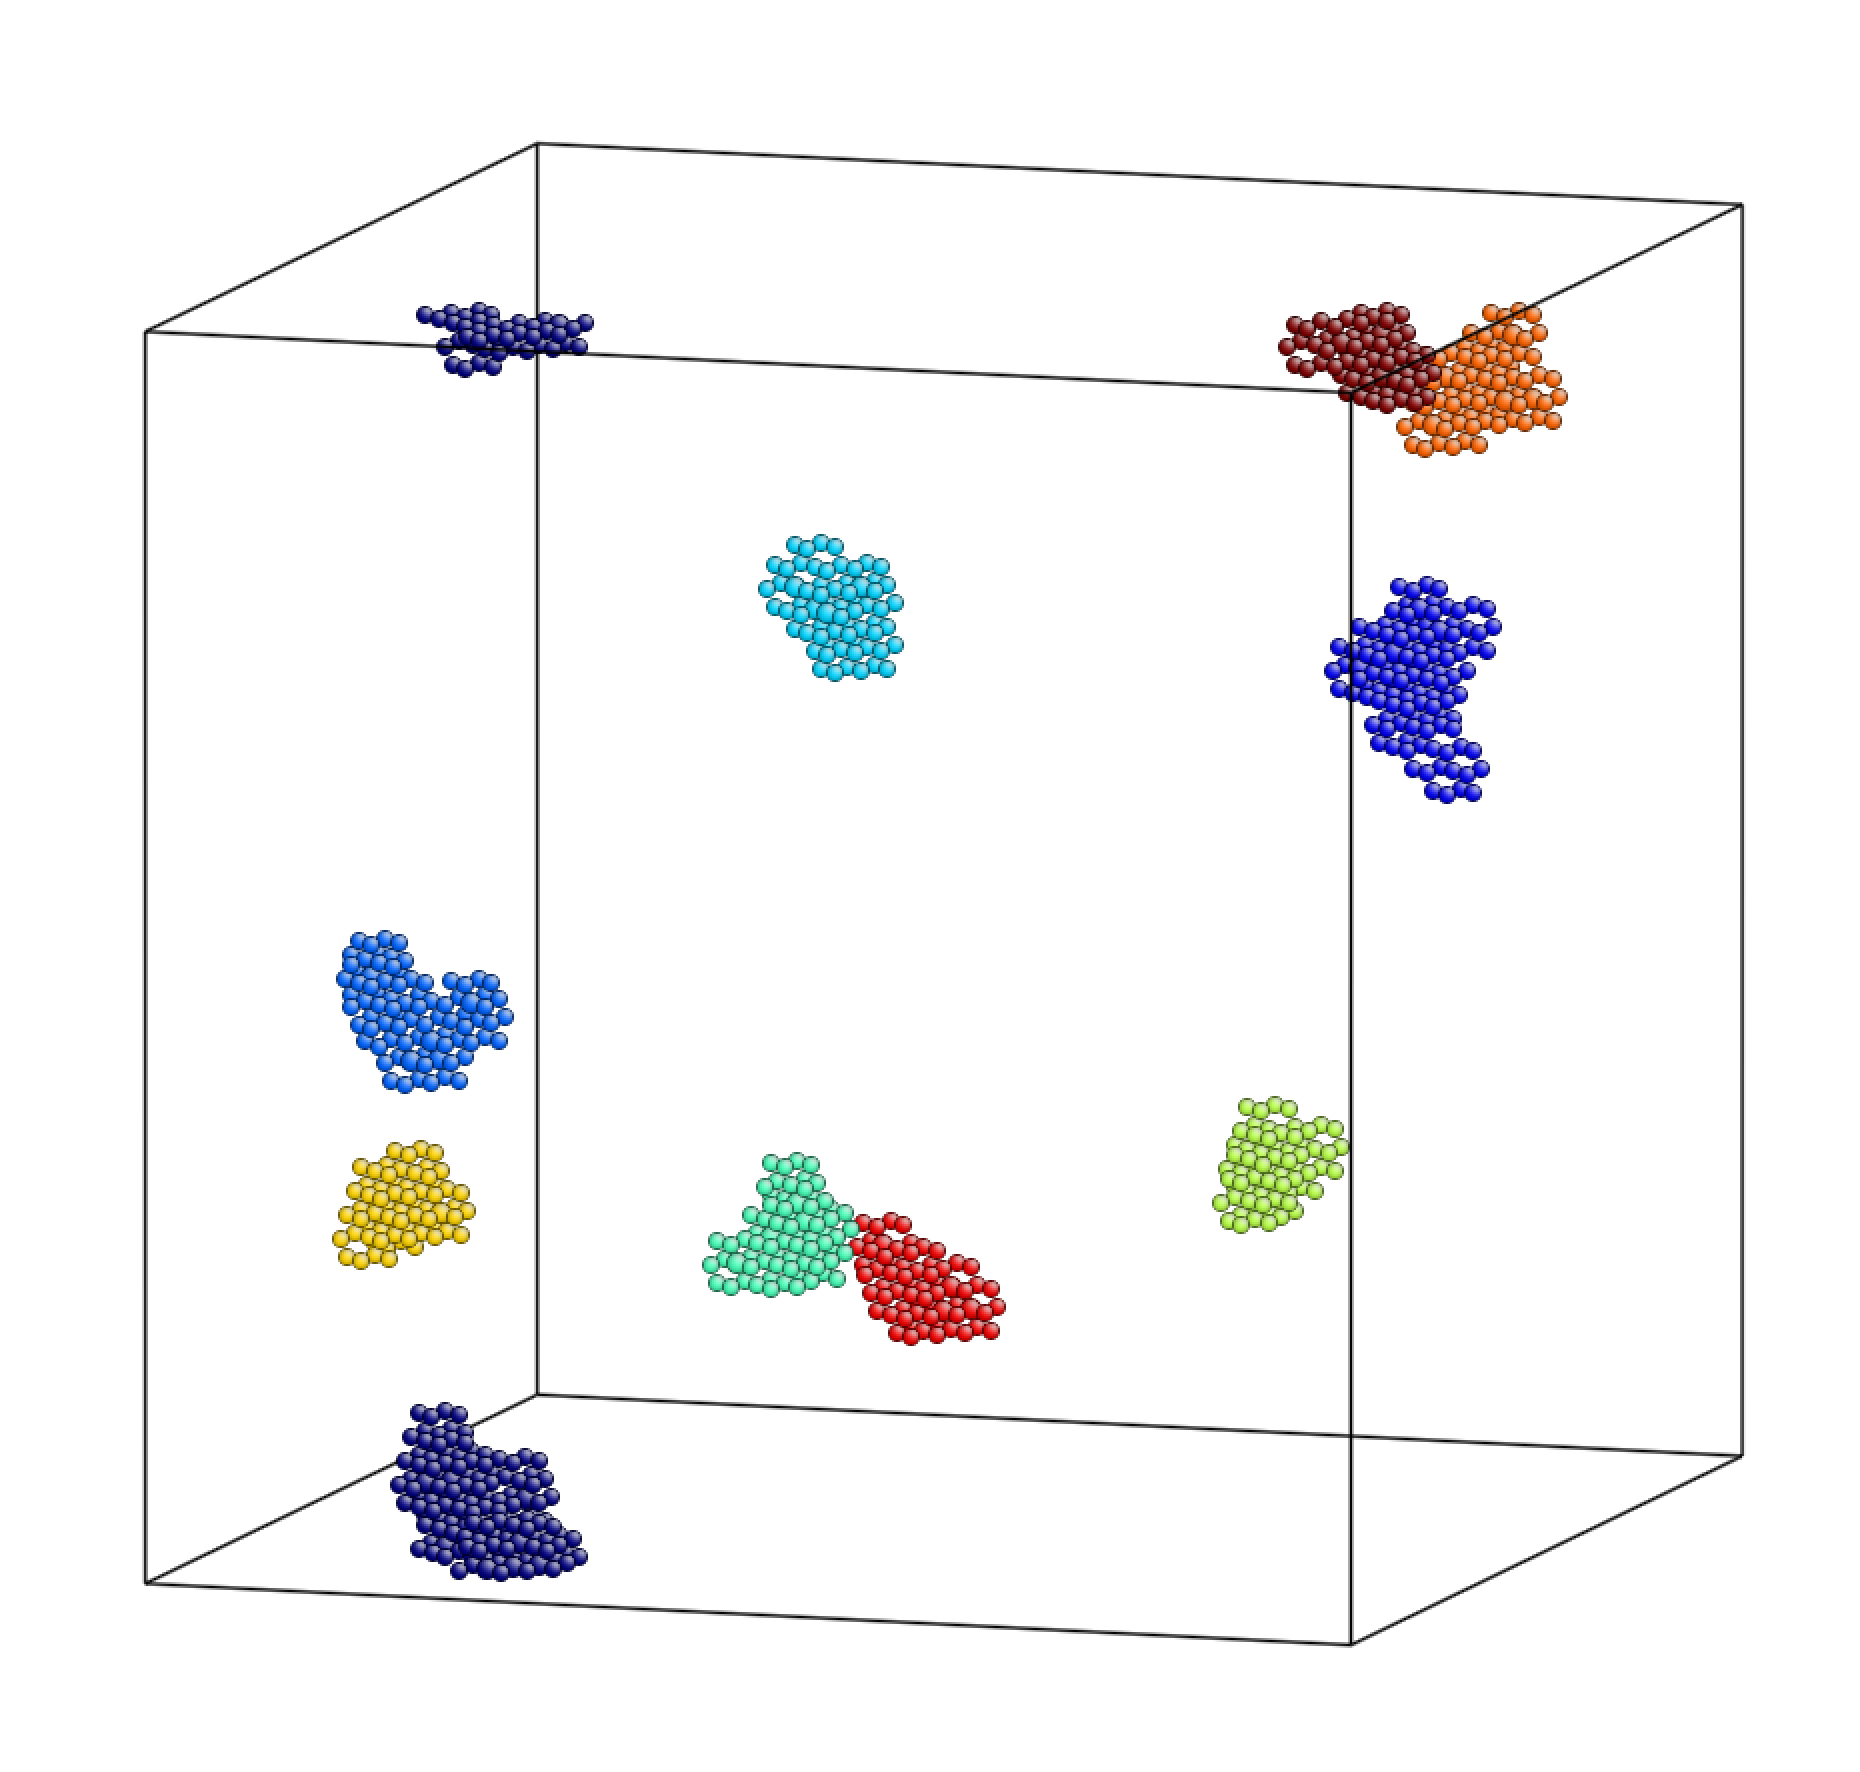
\includegraphics[width=0.45\linewidth]{Chap5/plots/cluster_illu_2.png}}
\caption[Atomistic pictures of top 10 clusters by size via cluster searching algorithm.]{Atomistic pictures of top 10 clusters by size via cluster searching algorithm. (a) Atomistic pictures of clusters coloring in atom species. Light green, dark green, and red atoms are Al, Mg, and Zn, respectively. (b) Atomistic pictures of clusters coloring in cluster id. The color mapping from dark blue to red is ranked by the cluster size in descending order.}
\label{Chap:Al/Vac:fig:illu_cluster}
\end{figure}
\endgroup


\subsection{Searching for Potential Elements that Can Slow Down Early Stage Nucleation}
